\chapter{How to Dive into a Code Base}
\label{chap:how-to-dive-into-a-code-base}

"Read the source" is one of the most annoying things to be told, but dealing with Erlang programmers, you'll have to do it often. Either the documentation for a library will be incomplete, outdated, or just not there. In other cases, Erlang programmers are a bit similar to Lispers in that they will tend to write libraries that will solve their problems and not really test or try them in other circumstances, leaving it to you to extend or fix issues that arise in new contexts.

It's thus pretty much guaranteed you'll have to go dive in some code base you know nothing about, either because you inherited it at work, or because you need to fix it or understand it to be able to move forward with your own system. This is in fact true of most languages whenever the project you work on is not one you designed yourself.

There are three main types of Erlang code bases you'll encounter in the wild: raw Erlang code bases, OTP applications, and OTP releases. In this chapter, we'll look at each of these and try to provide helpful tips on navigating them.

\section{Raw Erlang}
\label{sec:dive-raw-erlang}

If you encounter a raw Erlang code base, you're pretty much on your own. These rarely follow any specific standard, and you have to dive in the old way to figure out whatever happens in there.

This means hoping for a \filename{README.md} file or something similar that can point to an entry point in the application, and going from there, or hoping for some contact information that can be used to ask questions to the author(s) of the library.

Fortunately, you should rarely encounter raw Erlang in the wild, and they are often beginner projects, or awesome projects that were once built by Erlang beginners and now need a serious rewrite. In general, the advent of tools such as \app{rebar}\footnote{\href{https://github.com/rebar/rebar/}{https://github.com/rebar/rebar/} — a build tool briefly introduced in Chapter \ref{chap:building-open-source-erlang-software}} made it so most people use OTP Applications.

\section{OTP Applications}
\label{sec:dive-otp-applications}

Figuring out OTP applications is usually rather simple. They usually all share a directory structure that looks like:

\begin{VerbatimRaw}
doc/
ebin/
src/
test/
LICENSE.txt
README.md
rebar.config
\end{VerbatimRaw}

There might be slight differences, but the general structure will be the same.

Each OTP application should contain an \emph{app file}, either \filename{ebin/<AppName>.app} or more often, \filename{src/<AppName>.app.src}\footnote{A build system generates the final file that goes in \filename{ebin}. Note that in these cases, many  \filename{src/<AppName>.app.src} files do not specify modules and let the build system take care of it.}. There are two main varieties of app files:

\includecode[erlang]{useragent.app.src}

And:

\includecode[erlang]{dispcount.app}

This first case is called a \emph{library application}, while the second case is a regular \emph{application}.

\subsection{Library Applications}
\label{subsec:dive-library-applications}

Library applications will usually have modules named \module{\emph{appname}\_something}, and one module named \module{\emph{appname}}. This will usually be the interface module that's central to the library and contains a quick way into most of the functionality provided.

By looking at the source of the module, you can figure out how it works with little effort: If the module adheres to any given behaviour (\module{gen\_server}, \module{gen\_fsm}, etc.), you're most likely expected to start a process under one of your own supervisors and call it that way. If no behaviour is included, then you probably have a functional, stateless library on your hands. For this case, the module's exported functions should give you a quick way to understand its purpose.

\subsection{Regular Applications}
\label{subsec:dive-regular-applications}

For a regular OTP application, there are two potential modules that act as the entry point:

\begin{enumerate*}
	\item \module{\emph{appname}}
	\item \module{\emph{appname}\_app}
\end{enumerate*}

The first file should be similar in use to what we had in a library application (an entry point), while the second one will implement the \module{application} behaviour, and will represent the top of the application's process hierarchy. In some cases the first file will play both roles at once.

If you plan on simply adding the application as a dependency to your own app, then look inside \module{\emph{appname}} for details and information. If you need to maintain and/or fix the application, go for \module{\emph{appname}\_app} instead.

The application will start a top-level supervisor and return its \emph{pid}. This top-level supervisor will then contain the specifications of all the child processes it will start on its own\footnote{In some cases, the supervisor specifies no children: they will either be started dynamically by some function of the API or in a start phase of the application, or the supervisor is only there to allow OTP environment variables (in the \expression{env} tuple of the app file) to be loaded.}.

The higher a process resides in the tree, the more likely it is to be vital to the survival of the application. You can also estimate how important a process is by the order it is started (all children in the supervision tree are started in order, depth-first). If a process is started later in the supervision tree, it probably depends on processes that were started earlier.

Moreover, worker processes that depend on each other within the same application (say, a process that buffers socket communications and relays them to a finite-state machine in charge of understanding the protocol) are likely to be regrouped under the same supervisor and to fail together when something goes wrong. This is a deliberate choice, as it is usually simpler to start from a blank slate, restarting both processes, rather than trying to figure out how to recuperate when one or the other loses or corrupts its state.

The supervisor restart strategy reflects the relationship between processes under a supervisor:

\begin{itemize*}
	\item \expression{one\_for\_one} and \expression{simple\_one\_for\_one} are used for processes that are not dependent upon each other directly, although their failures will collectively be counted towards total application shutdown\footnote{Some developers will use \expression{one\_for\_one} supervisors when \expression{rest\_for\_one} is more appropriate. They require strict ordering to boot correctly, but forget about said order when restarting or if a predecessor dies.}.
	\item \expression{rest\_for\_one} will be used to represent processes that depend on each other in a linear manner.
	\item \expression{one\_for\_all} is used for processes that entirely depend on each other.
\end{itemize*}

This structure means it is easiest to navigate OTP applications in a top-down manner by exploring supervision subtrees. 

For each worker process supervised, the behaviour it implements will give a good clue about its purpose:

\begin{itemize*}
	\item a \module{gen\_server} holds resources and tends to follow client/server patterns (or more generally, request/response patterns)
	\item a \module{gen\_fsm} will deal with a sequence of events or inputs and react depending on them, as a Finite State Machine. It will often be used to implement protocols.
	\item a \module{gen\_event} will act as an event hub for callbacks, or as a way to deal with notifications of some sort.
\end{itemize*}

All of these modules will contain the same kind of structure: exported functions that represent the user-facing interface, exported functions for the callback module, and private functions, usually in that order.

Based on their supervision relationship and the typical role of each behaviour, looking at the interface to be used by other modules and the behaviours implemented should reveal a lot of information about the program you're diving into.

\subsection{Dependencies}
\label{subsec:dive-dependencies}

All applications have dependencies\footnote{At the very least on the \module{kernel} and \module{stdlib} applications}, and these dependencies will have their own dependencies. OTP applications usually share no state between them, so it's possible to know what bits of code depend on what other bits of code by looking at the app file only, assuming the developer wrote them in a mostly correct manner. Figure~\ref{fig:app-deps} shows a diagram that can be generated from looking at app files to help understand the structure of OTP applications.


\begin{figure}
  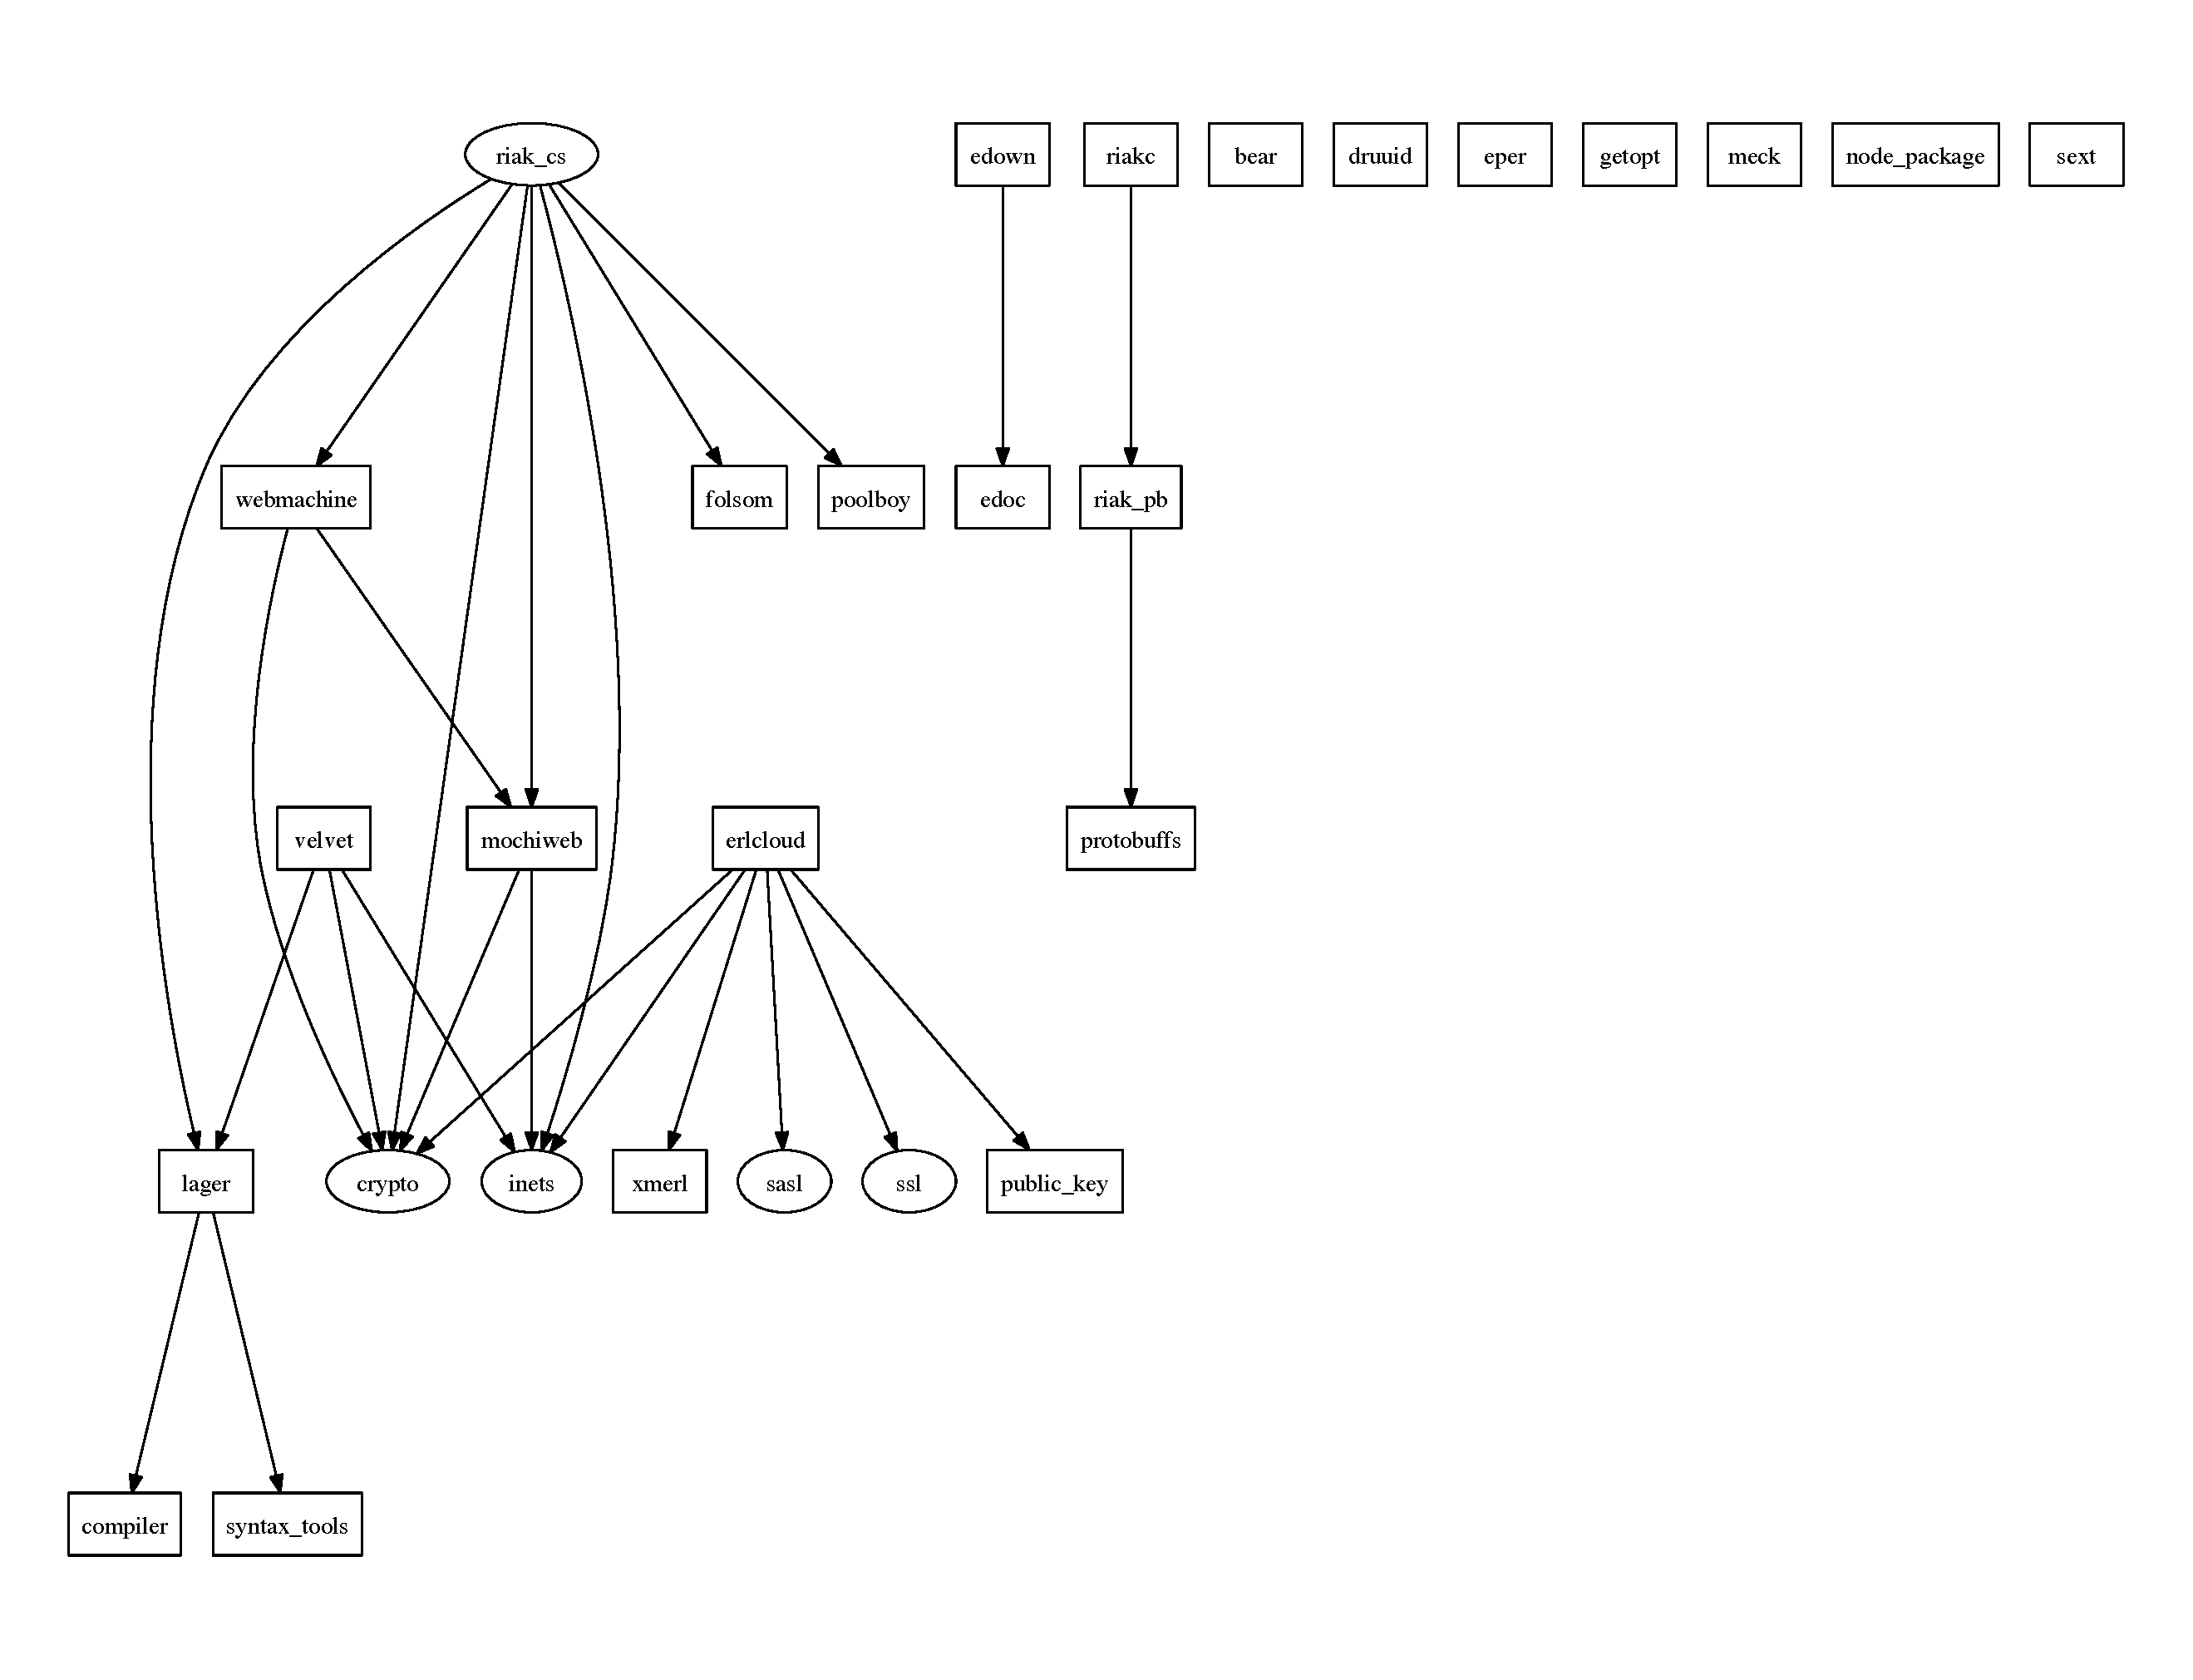
\includegraphics{app-deps-riak-cs.pdf}%
  \caption{Dependency graph of riak\_cs, Basho's open source cloud library.
  The graph ignores dependencies on common applications like kernel and stdlib. Ovals are applications, rectangles are library applications.}%
   \label{fig:app-deps}
\end{figure}

Using such a hierarchy and looking at each application's short description might be helpful to draw a rough, general map of where everything is located. To generate a similar diagram, find \app{recon}'s script directory and call \command{escript script/app\_deps.erl}\footnote{This script depends on graphviz}. Similar hierarchies can be found using the \module{observer}\footnote{\href{http://www.erlang.org/doc/apps/observer/observer\_ug.html}{http://www.erlang.org/doc/apps/observer/observer\_ug.html}} application, but for individual supervision trees. Put together, you may get an easy way to find out what does what in the code base.

\FloatBarrier

\section{OTP Releases}
\label{sec:dive-otp-releases}

OTP releases are not a lot harder to understand than most OTP applications you'll encounter in the wild. A release is a set of OTP applications packaged in a production-ready manner so it boots and shuts down without needing to manually call \function{application:start/2} for any app. Of course there's a bit more to releases than that, but generally, the same discovery process used for individual OTP applications will be applicable here.

You'll usually have a file similar to the configuration files used by \module{systools} or \module{reltool}, which will state all applications part of the release and a few\footnote{A lot} options regarding their packaging. To understand them, I recommend \href{http://learnyousomeerlang.com/release-is-the-word}{reading existing documentation on them}. If you're lucky, the project may be using \app{relx}\footnote{\href{https://github.com/erlware/relx/wiki}{https://github.com/erlware/relx/wiki}}, an easier tool that was officially released in early 2014.


\section{Exercises}

\subsection*{Review Questions}

\begin{enumerate}
	\item How do you know if a code base is an application? A release?
	\item What differentiates an application from a library application?
	\item What can be said of processes under a \term{one\_for\_all} scheme for supervision?
	\item Why would someone use a \module{gen\_fsm} behaviour over a \module{gen\_server}?
\end{enumerate}

\subsection*{Hands-On}

Download the code at \href{https://github.com/ferd/recon\_demo}{https://github.com/ferd/recon\_demo}. This will be used as a test bed for exercises throughout the book. Given you are not familiar with the code base yet, let's see if you can use the tips and tricks mentioned in this chapter to get an understanding of it.

\begin{enumerate}
	\item Is this application meant to be used as a library? A standalone system?
	\item What does it do?
	\item Does it have any dependencies? What are they?
	\item The app's \filename{README} mentions being non-deterministic. Can you prove if this is true? How?
	\item Can you express the dependency chain of applications in there? Generate a diagram of them?
	\item Can you add more processes to the main application than those described in the \filename{README}? 
\end{enumerate}

